\begin{frame}{Introduction}
	The Capacitated Vehicle Routing Problem (\textbf{CVRP}) \parencite{dantzig1959}
	is an \textcolor{blue}{NP-hard combinatorial optimization routing problem} with applications in \textcolor{blue}{logistics} (transportation, distribution, delivery).

	\vspace{0.25cm}

	\begin{columns}
		\begin{column}{.35\textwidth}
			\centering
			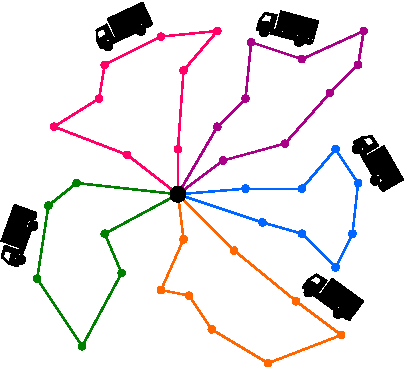
\includegraphics[height=4cm]{Imgs/CVRP-example.cropped.pdf}
		\end{column}
		\begin{column}{.65\textwidth}
			\onslide<+->{
				\begin{itemize}[<+->]
					\item CVRP defined on a complete graph. We are given:
					      \begin{itemize}[<.->]
						      \item The amount of \textcolor{blue}{available vehicles} with their \textcolor{blue}{capacity}.
						      \item A \textcolor{blue}{central depot} where vehicles are stationed.
						      \item Customers' \textcolor{blue}{locations}.
						      \item The \textcolor{blue}{demands} (in units) of the individual customers.
					      \end{itemize}

					\item Objective:
					      \begin{itemize}[<.->]
						      \item \textcolor{red}{Minimize overall routing costs while meeting the needs of \textbf{all} customers.}
					      \end{itemize}
				\end{itemize}
			}
		\end{column}
	\end{columns}
\end{frame}

\begin{frame}{Branch-price-and-cut}
	\onslide<+->{
		\begin{columns}
			\begin{column}{.7\textwidth}
				\begin{itemize}
					\item In the last two decades, the most efficient VRP solvers are all based on branch-price-and-cut approaches \cite{fukasawa2006, pessoa2008, gutierrez-jarpa2010, archetti2011, bettinelli2011, contardo2014, contardo2015, pecin2017new, pecin2017improved, pessoa2020generic}.
					\item \textcolor{blue}{Branch-price-and-cut} (BPC) is an \textbf{exact approach} for solving combinatorial optimization problems.
					      \begin{itemize}
						      \item Extension of traditional \textcolor{blue}{branch-and-cut} (BAC).
						      \item Can tackle \textcolor{blue}{\textbf{extensive} integer programming models}.
					      \end{itemize}
				\end{itemize}
			\end{column}
			\begin{column}{.3\textwidth}
				{
					\fontsize{9.5pt}{9.5pt}\selectfont

					\begin{align*}
						\min_{\lambda} \quad z_\mt{SC}(\lambda) & = \sum_{p \in P}  c_p \lambda_p                                      \\
						                                        & \sum_{p \in P} \lambda_{p} = K                                       \\
						                                        & \sum_{p \in P}  a_{ip} \lambda_p \ge 1       \quad \forall i \in V_0 \\
						                                        & \lambda_p                    \in \Set*{0, 1} \quad \forall p \in P.
					\end{align*}
				}
			\end{column}
		\end{columns}
	}

	\onslide<+->{
		\begin{itemize}
			\item \textcolor{red}{How?}
			      \begin{itemize}
				      \item \textcolor{blue}{Column Generation} (CG): decision variables are generated lazily.
				            \begin{itemize}
					            \item In VRP, decision variables represent \textcolor{blue}{single vehicle feasible routes}.
				            \end{itemize}
				      \item \textcolor{red}{\textbf{Pricing}}: determines the optimal \textcolor{blue}{reduced-cost decision variables} for their inclusion.
			      \end{itemize}
		\end{itemize}
	}
\end{frame}

\begin{frame}{Contemporary Approaches for Pricing}
	\begin{itemize}[<+->]
		\item Pricing Problem (PP) in its "natural" form is an induced \textbf{NP-hard} combinatorial optimization problem \parencite{dror1994}.
		      \begin{itemize}[<.->]
			      \item An \textcolor{blue}{Elementary Shortest Path Problem with Resource Constraints} (\textbf{ESPPRC}) in a reduced cost network with negative cycles:
		      \end{itemize}
		      \begin{equation}\label{eq:pp-problem}
			      {c^\star_p} = \min_{p \in P} \Set*{ \bar{c}_p = \sum_{e = \Set*{i, j} \in E} \Expr*{c_{e} - \frac{\pi_i + \pi_j}{2}} a_{ep}  }.
		      \end{equation}
		\item PP hard $\,\to\,$ \textcolor{olive}{Relaxation} of the PP.
		      \begin{itemize}[<.->]
			      \item \textcolor{olive}{Relaxed} PP is solvable in \textcolor{blue}{pseudo-polynomial time} \parencite{desrochers1988, irnich2005} via efficient \textcolor{blue}{dynamic programming} algorithms.
			            \begin{itemize}[<.->]
				            \item \textbf{Labeling algorithm} proposed in \citeyear{desrochers1992} in \cite{desrochers1992}.
				            \item Labeling algorithm extended to handle elementarity condition in \citeyear{feillet2004} in \cite{feillet2004}.
			            \end{itemize}
		      \end{itemize}
	\end{itemize}
\end{frame}

\begin{frame}{Issues with Contemporary Approaches}
	\textcolor{red}{\textbf{Two major issues with contemporary approaches}}:
	\begin{enumerate}
		\item (weak) \textcolor{olive}{relaxing} the PP weakens the dual bounds fed to the BPC (increasing column generation time).
		      \begin{itemize}[<.->]
			      \item \textcolor{blue}{Recently alleviated} thanks to recent developments of \textcolor{olive}{efficacious relaxations} \parencite{baldacci2011}.
		      \end{itemize}
		\item (strong) \textbf{Labeling} algorithm's performance degrades as the \textcolor{blue}{vehicle capacity increases} $O(N^2 Q)$ (longer routes), limiting its applicability to modern distribution problems.
	\end{enumerate}
\end{frame}

\begin{frame}{Contributions}
	\begin{columns}
		\begin{column}{0.3\textwidth}
			\centering
			
\includegraphics[width=\textwidth]{./Imgs/idea.png}
		\end{column}
		\begin{column}{0.7\textwidth}
			\begin{enumerate}
				\item An exact \textcolor{blue}{branch-and-cut} approach for the \textcolor{olive}{\textbf{non}-relaxed} pricing problem.
				      \begin{itemize}
					      \item Almost no works on this domain, except \parencite{jepsen2014}.
				      \end{itemize}
				\item We compare its competitiveness against state-of-the-art solutions as the \textcolor{blue}{vehicle capacity increases}.
			\end{enumerate}
		\end{column}
	\end{columns}
\end{frame}

\begin{frame}{Implementation}
	\begin{columns}
		\begin{column}{0.85\textwidth}
			\begin{itemize}
				\item Available online\footnote[1]{\url{https://github.com/dparo/master-thesis}} under a permissive license.
				\item Implemented in \texttt{C} using the commercial \textcolor{blue}{IBM ILOG CPLEX optimizer}.
				\item The \textbf{Capacitated Profitable Tour Problem} (CPTP) \parencite{jepsen2014} was used as the base IP formulation to model the PP.

			\end{itemize}
		\end{column}
		\begin{column}{0.15\textwidth}
			\centering
			
\includegraphics[width=\textwidth]{./Imgs/IBM-ILOG-CPLEX-logo.png}
		\end{column}
	\end{columns}

	\vspace{0.2cm}

	\begin{itemize}
		\item Some implementation details:
		      \begin{itemize}
			      \item Heuristics for warm-starting (constructive + local-search).
			      \item Inclusion of several \textcolor{blue}{cutting-planes}:
			            \begin{itemize}
				            \item GSEC, RCC \parencite{laporte1983}, GLM \parencite{gouveia1995}.
				            \item Integral separation by tracking major connected components.
				            \item Fractional separation through push relabel max-flow \parencite{goldberg1997} and Gomory-Hu trees \parencite{gomory1961}.
			            \end{itemize}
		      \end{itemize}
	\end{itemize}
\end{frame}

\begin{frame}{Empirical evaluation}
	\begin{columns}
		\begin{column}{0.2\textwidth}
			\centering
			
\includegraphics[width=\textwidth]{./Imgs/testing.png}
		\end{column}
		\begin{column}{0.8\textwidth}
			\begin{itemize}
				\item We've modified the commonly employed traditional instances proposed in
				      \cite{dantzig1959, christofides1969, gaskell1967bases, gillett1974heuristic,christofides1979vehicle,fisher1994,augerat1995}.
				\item \bapcod{}: State-of-the-art BPC of \cite{sadykov2021bucket} developed in France at the Bordeaux University and Bordeaux Research Center.
				      \begin{itemize}
					      \item Parametrized accordingly (disabled non-robust inequalities).
				      \end{itemize}
				\item Time the \bapcod{}'s labeling algorithm \cite{pessoa2020generic} and our BAC in solving the harder PPs.
				\item Running time depicted through \textbf{performance profiles} \parencite{dolan2002}.
			\end{itemize}
		\end{column}
	\end{columns}
\end{frame}

\newcommand{\IncludeTimeProfile}[1]{
	\centering
	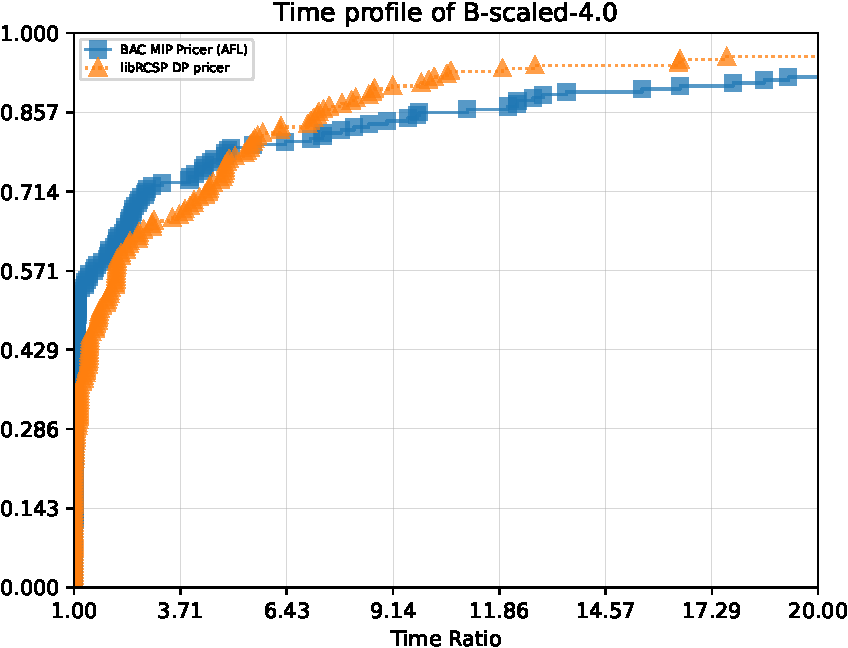
\includegraphics[height=6.5cm]{./Imgs/perfprofs/#1/Time_plot.cropped.pdf}
}

\newcommand{\IncludeDualBounds}[1]{
	\centering
	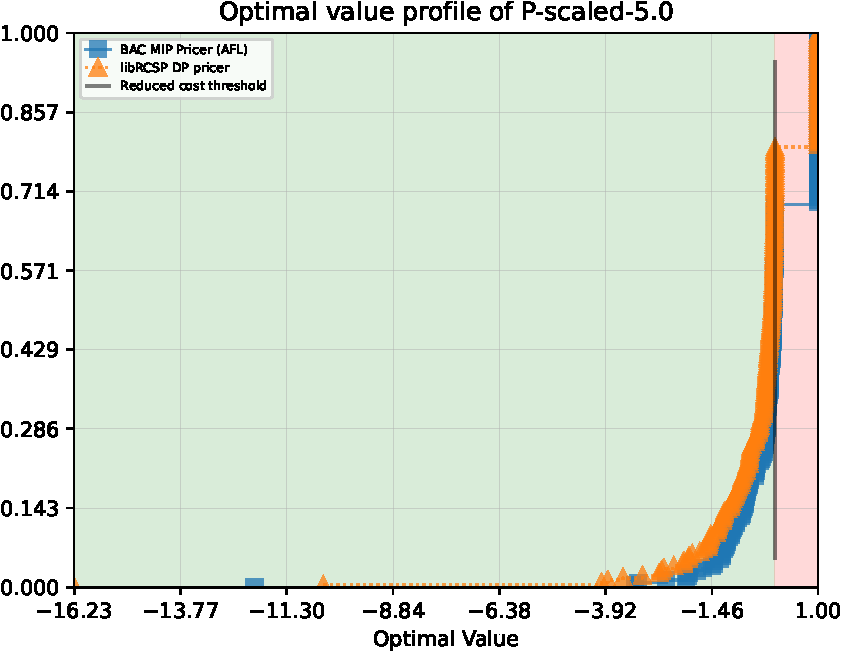
\includegraphics[width=1.0\linewidth]{./Imgs/perfprofs/#1/OptimalValue_plot.cropped.pdf}
}

\begin{frame}{Results (1/2)}
	\IncludeTimeProfile{E-scaled-1.0}
\end{frame}
\begin{frame}
	\IncludeTimeProfile{E-scaled-4.0}
\end{frame}
\begin{frame}
	\IncludeTimeProfile{E-scaled-8.0}
\end{frame}
\begin{frame}
	\IncludeTimeProfile{E-scaled-20.0}
\end{frame}

\begin{frame}{Results (2/2)}
	\begin{columns}
		\begin{column}{0.25\textwidth}
			\IncludeDualBounds{E-scaled-1.0}
		\end{column}
		\begin{column}{0.25\textwidth}
			\IncludeDualBounds{E-scaled-4.0}
		\end{column}
		\begin{column}{0.25\textwidth}
			\IncludeDualBounds{E-scaled-8.0}
		\end{column}
		\begin{column}{0.25\textwidth}
			\IncludeDualBounds{E-scaled-20.0}
		\end{column}
	\end{columns}
	\begin{columns}
		\begin{column}{0.25\textwidth}
			\IncludeDualBounds{F-scaled-1.0}
		\end{column}
		\begin{column}{0.25\textwidth}
			\IncludeDualBounds{F-scaled-4.0}
		\end{column}
		\begin{column}{0.25\textwidth}
			\IncludeDualBounds{F-scaled-8.0}
		\end{column}
		\begin{column}{0.25\textwidth}
			\IncludeDualBounds{F-scaled-20.0}
		\end{column}
	\end{columns}

\end{frame}

\begin{frame}{Conclusions and Future Work}
	The proposed branch-and-cut pricer proved competitive at solving some PP:
	\begin{itemize}
		\item \textcolor{blue}{Branch-and-cut} approaches may supplement the traditional \textcolor{blue}{labeling algorithm}.
		\item Suggesting future research on \textcolor{blue}{branch-and-cut} approaches in the context of \textbf{pricing for the CVRP}.
		      Benefits:
		      \begin{itemize}
			      \item Improve performance of contemporary CVRP solvers.
		      \end{itemize}
	\end{itemize}
\end{frame}

\begin{frame}{The end}
	\begin{center}
		\begingroup
		\fontsize{18pt}{18pt}\selectfont
		Thank you all!
		\endgroup
	\end{center}
\end{frame}

\appendix

\begin{frame}
\end{frame}

\begin{frame}
	\begin{center}
		\begingroup
		\fontsize{18pt}{18pt}\selectfont
		Additional material.
		\endgroup
	\end{center}
\end{frame}

\begin{frame}{Integer Programming}
	MIP solvers are rather general and can be used to solve a wide range of problems from various fields \parencite{bixby2007progress}.
	MIP models are, in spirit, a way to mathematically program a solver to achieve the desired solution.
	A MIP solver can solve a mixed-integer linear programming formulation
	expressed as \parencite{wolsey1999integer}:
	\begin{align}
		 & \max_{x, y} & c^T x + d^T y                                 \\
		 & \text{s.t.} & A x + B y \le b  \label{eq:general-mip-bound} \\
		 &             & x \in \R^n                                    \\
		 &             & y \in \Z_{+}^k,
	\end{align}
	where $A \in \R^{m \times n}, B \in \R^{m \times k}$ are matrices and
	$c \in \R^n, d \in R^k, b \in \R^m$ are vector coefficients.
	The bound in \cref{eq:general-mip-bound} can also be rewritten in equality and/or greater form.
\end{frame}

\begin{frame}{History on CVRP exact solvers}
	\begin{itemize}
		\item 1959: The CVRP was first introduced in \cite{dantzig1959}.
		\item 1961: First branch-and-price applied to the Cutting Stock Problem in \cite{gilmore1961}.
		\item Up to late 80s: tree search algorithms employing branch-and-bound schemes: Lagrangian duality relaxation, \dots.
		\item Mid 80s: First Column Generation attempts \parencite{desrosiers1984, agarwal1989setpartitioningbased}.
		\item From late 80s to first 2000s: branch-and-cut approaches \cite{laporte1983, laporte1985, augerat1995approche, araqueg1994, augerat1995, achuthan1996, blasum2000, ralphs2003, achuthan2003, baldacci2004}.
		\item 1992: labeling algorithm for pricing in \cite{desrochers1992}.
		\item 1999: basic implementation of a BPC framework in \cite{kohl1999}.
		\item 2006: Turning point in modern BPC frameworks thanks to \parencite{fukasawa2006}.
		\item 2011: smart ng-routes relaxation for the pricing problem \parencite{baldacci2011}.
		\item 2014-now: State-of-the-art BPC algorithms \parencite{contardo2014,pecin2017improved,pecin2017new,pessoa2020,sadykov2021,pessoa2020generic}.
	\end{itemize}
\end{frame}

\begin{frame}{Set Covering formulation}
	Let $P = \Set*{p \mid p\ \text{is a single-truck elementary feasible route}}$ be the set of all feasible routes.

	\begin{align}
		\min_{\lambda} \quad z_\mt{SC}(\lambda) & = \sum_{p \in P}  c_p \lambda_p              & \label{eq:set-covering-obj-func}                                                       \\
		                                        & \sum_{p \in P} \lambda_{p} = K               & \label{eq:set-covering-K-routes}                                                       \\
		                                        & \sum_{p \in P}  a_{ip} \lambda_p \ge 1       & \quad \forall i \in V_0 \label{eq:set-covering-customers-visited-by-exactly-one-route} \\
		                                        & \lambda_p                    \in \Set*{0, 1} & \quad \forall p \in P \label{eq:set-covering-lambda-mip-var-bounds}.
	\end{align}
\end{frame}

\begin{frame}{Master Problem (Primal)}
	\begin{align}
		\min_{\lambda} \quad z_\mt{MP}(\lambda) & = \sum_{p \in P}  c_p \lambda_p      & \label{eq:mp-obj-func}                                                                                                    \\
		                                        & \sum_{p \in P} \lambda_{p} = K       & \label{eq:mp-K-routes}                                                                                                    \\
		                                        & \sum_{p \in P}  a_{ip} \lambda_p = 1 & \quad \forall i \in V_0                                              \label{eq:mp-customers-visited-by-exactly-one-route} \\
		                                        & 0 \le \lambda_p \le 1                & \quad \forall p \in P \label{eq:mp-lambda-mip-var-bounds}.
	\end{align}
\end{frame}

\begin{frame}{Master Problem (Dual)}
	\begin{align}
		\max_{\pi} \quad z_\mt{DMP}(\pi) & =  K \pi_0 + \sum_{i \in V_0} \pi_i           & \label{eq:dmp-obj-func}                             \\
		                                 & \pi_0 + \sum_{i \in V_0} a_{ip} \pi_i \le c_p & \quad \forall p \in P \label{eq:dmp-constraint1}    \\
		                                 & \pi_0 \in \R                                  & \label{eq:dmp-constraint2}                          \\
		                                 & \pi_i \in \R                                  & \quad \forall i \in V_0 \label{eq:dmp-constraint3},
	\end{align}
	where $\pi_0 \in \R, \pi_i \in \R \quad \forall i \in V_0$ represents the dual variables
	associated respectively with constraints \labelcref{eq:mp-K-routes,eq:mp-customers-visited-by-exactly-one-route}.
\end{frame}

\begin{frame}{Restricted Master Problem}
	Due to the enormous size of the set of routes $P$, evaluating the dual variables $\pi \in \R^{N}$ is computationally intractable.
	As a result, in BAP frameworks we consider only a small subset of columns $\mcP \subseteq P$:
	\begin{align}
		\min_{\lambda} \quad z_\mt{RMP}(\lambda) & = \sum_{p \in \mcP}  c_p \lambda_p      & \label{eq:rmp-obj-func}                                                                                                    \\
		                                         & \sum_{p \in \mcP} \lambda_{p} = K       & \label{eq:rmp-K-routes}                                                                                                    \\
		                                         & \sum_{p \in \mcP}  a_{ip} \lambda_p = 1 & \quad \forall i \in V_0                                              \label{eq:rmp-customers-visited-by-exactly-one-route} \\
		                                         & \lambda_p \ge 0                         & \quad \forall p \in \mcP \label{eq:rmp-lambda-mip-var-bounds}.
	\end{align}
\end{frame}

\begin{frame}{Pricing sub-problem}
	We look for a column to enter the basis of the RMP,
	which in turn necessitates the resolution of the following sub-problem:
	\begin{equation}\label{eq:pp-problem-2nd-time}
		{c^\star_p} = \min_{p \in P} \Set*{ \bar{c}_p = \sum_{e = \Set*{i, j} \in E} \Expr*{c_{e} - \frac{\pi_i + \pi_j}{2}} a_{ep}  },
	\end{equation}
	which takes the name of \textit{Pricing Problem} (PP).
	Any $p \in P$ which satisfies $c_p < 0$ is a valid column which can enter the basis of the RMP.
	The column generation procedure stops mainly under two scenarios:
	(i) when no more negative reduced cost routes exist,
	i.e. the PP outputs a $p^\star \in P$ achieving $c^\star_p \ge 0$
	or
	(ii) the CG procedure tails off.

\end{frame}

\begin{frame}{Pricing Sub-problem Relaxations}
	\begin{itemize}
		\item \textbf{Relax elementarity condition} to make the PP solvable in pseudo-polynomial time:
		      \begin{itemize}
			      \item $q$-routes with 2-cycles elimination \parencite{christofides1981exact}.
			      \item $q$-routes with arbitrary $k$-cycles elimination \parencite{feillet2004, chabrier2006}.
			      \item ng-routes \parencite{baldacci2011}.
		      \end{itemize}
	\end{itemize}
\end{frame}

\begin{frame}{CPTP}
	\begin{align}
		\min_{x,y} \quad z_\mt{CPTP}(x, y) & = \ExprCptpObjValDef                     & \label{eq:cptp-obj-function}                                                                          \\
		                                   & y_0 = 1                                  & \label{eq:cptp-depot-part-of-tour-constraint}                                                         \\
		                                   & \ExprCptpDemandSum  \le Q                & \label{eq:cptp-resource-upper-bound-constraint}                                                       \\
		                                   & \ExprCptpEdgesIncident{i}  = 2 y_i       & \quad \forall i \in V         \label{eq:cptp-flow-conservation-constraint}                            \\
		                                   & \ExprCptpFlowExiting{S} \ge 2 y_{i}      & \quad \forall i \in S,\ \forall S \subseteq V_0,\ \SetSize*{S} \ge 2 \label{eq:cptp-gsec-constraints} \\
		                                   & x_{e}                   \in \Set*{0, 1}  & \quad \forall e \in E               \label{eq:cptp-x-mip-var-bounds}                                  \\
		                                   & y_{i}                    \in \Set*{0, 1} & \quad \forall i \in V             \label{eq:cptp-y-mip-var-bounds}.
	\end{align}
\end{frame}
